\section{Arquitetura Implementada}

Nesta Secção iremos descrever a arquitetura que implementámos para obter uma infraestrutura de elevada disponibilidade e desempenho, explicando quais as ferramentas utilizadas e explicando como estas resolvem os problemas identificados anteriormente. De modo a comparar a arquitetura implementada com a anterior, iremos efetuar os mesmos testes de carga de modo a comparar as duas soluções para poder efetuar comparações.

\subsection{Camada de Persistência}

Para a camada de persistência do sistema, iremos apresentar as componentes que a constituem pela ordem de implementação. 

A primeira componente desta camada consiste num grupo de VM's que constituem um \textbf{DRBD} (\textit{Distributed Replicated Block Device}) que são acedidas utilizando o protocolo \textbf{iSCSI} (\textit{Internet Small Computer Systems Interface}). Para esta componente criámos \textbf{duas instâncias de VM} na GCP com \textbf{2 vCPU} e \textbf{4GB de memória}. Cada uma das máquinas possui um disco \textbf{SSD de 20GB} onde foi instalado o sistema operativo (CentOS 8). A utilização de DRBD deve-se ao facto de este permitir garantir a replicação dos nossos dados. Para o armazenamento dos dados, cada uma das instâncias possui um \textbf{disco SSD de 50 GB} que irá ser atribuída a um recurso DRBD, sendo que o denominámos de \textbf{d1}. Ambas as instâncias foram sinalizadas como primárias para permitir que estas sejam utilizadas sem qualquer tipo de restrição. Para finalizar, numa das instâncias foi colocado um sistema de ficheiros no formato xfs, sendo estas alterações sincronizadas com a segunda instância. Após finalizada o setup do DRBD, avançámos para o setup do iSCSI \textit{target}.

A segunda componente desta camada consiste num grupo de VM's que constituem um cluster de elevada disponibilidade. Este cluster é constituído por \textbf{3 nodos}, tendo cada um \textbf{2 vCPU} e \textbf{8GB de memória}. Cada uma das máquinas possui um disco \textbf{SSD de 20GB} onde foi instalado o sistema operativo (CentOS 8). Cada uma das instâncias foi configurada com o cliente \textbf{iSCSI}, ligando-se a cada um dos \textit{targets}. Após esta configuração do iSCSI foi colocado um serviço \textbf{multipath}. De seguida foi feito o setup do \textbf{\textit{High-Availability Cluster}} da RedHat em cada uma das três instâncias, sendo este cluster composto por três nodos: \textbf{cluster1}, \textbf{cluster2} e \textbf{cluster3}. Neste cluster foram definidos dois serviços: o serviço \textbf{fs}, que consiste no sistema de ficheiros replicado anteriormente criado, e o serviço \textbf{bd}, que consiste na configuração da base de dados postgres que pretendemos manter.

A terceira e última componente que compõe a camada de persistência é um \textbf{\textit{(tcp) load balancer}} interno, que tem como principal função encaminhar os pedidos para o nó \textit{director} e, também, verificar se cada um dos nós do cluster se encontra operacional. Na eventualidade de o nó ativo ficar inoperacional, o \textit{load balancer} automaticamente comunica com o nó seguinte. Para conseguir isto agrupámos os nós do cluster em dois grupos: um grupo primário e um grupo secundário. O cluster1 foi adicionado ao grupo primário, sendo este o principal nodo do cluster. O cluster2 e o cluster3 foram adicionados ao grupo secundário, sendo que no caso do nodo principal falhar, o \textit{failover} é feito para um destes nodos. 

O acesso a esta camada de persistência é então feito a partir do \textit{load balancer}. Deste modo, possuímos uma camada de persistência que nos garante elevada disponibilidade bem como replicação do disco com os dados, isto é, no caso de um dos elementos que compõe esta camada falhar, o serviço não é interrompido, e no caso de um dos discos de armazenamento falhar, possuímos uma cópia de todos os dados, mantendo-se o serviço sem interrupções. Com a utilização de discos SSD somos capazes de implementar melhorias de \textit{performance}, tornando o nosso sistema mais rápido no geral.


\subsection{Camada Aplicacional}
A camada aplicacional tem a responsabilidade de tratar os pedidos e responder-lhes devidamente. Tal como se pode ver na figura \ref{fig:final-arch}, para esta camada decidiu-se ter três servidores semelhantes, cada um com a aplicação \textit{Wiki.js} instalada. Tanto para a camada aplicacional como para a camada web, decidiu-se ter VMs semelhantes com:

\pagebreak

\begin{itemize}
\item 2 CPUs;
\item 8 GB de Memória RAM;
\item 10 GB de disco;
\item Sistema operativo Ubuntu 20.04 LTS.
\end{itemize}

A razão para ter 3 servidores semelhantes na camada aplicacional serve o propósito de uma maior paralelização no atendimento de pedidos, o que de um modo geral permite diminuir os tempos de resposta, isto é, tornar as operações mais rápidas e distribuir a carga para várias instâncias da aplicação, ao invés de sobrecarregar uma única instância da aplicação.

A razão anterior foca-se no desempenho, outra razão tem que ver com elevada disponibilidade, pois, se um dos servidores entrar em falta e não for capaz de responder a pedidos, temos os outros dois servidores a responder. No limite, podem entrar em falta 2 dos 3 servidores aplicacionais. No caso dos 3 servidores falharem, o serviço fica indisponível.

Como nota final relativamente ao \textit{deployment} desta camada, para facilitar a manutenção das aplicações, em cada VM criou-se um serviço associado à aplicação, que foi utilizado para pôr as aplicações a correr e que facilita qualquer tipo de manutenção das mesmas através das premissas de \textit{enable}, \textit{disable}, \textit{start}, \textit{stop}, \textit{restart}, etc dos serviços \textit{Linux}. 

\subsection{Camada Web (\textit{Load Balancers})}
A camada mais superficial (mais próxima da \textit{Internet}) é a camada \textit{web}. Esta tem a responsabilidade de receber os pedidos e distribuí-los pelos vários servidores aplicacionais existentes (\textit{load balancer} e \textit{reverse proxy}), bem como controlar o tráfego, através de regras de \textit{firewall}.

Esta camada dividi-se em duas sub-camadas:
\begin{itemize}
\item Um load balancer externo que serve como ponto de acesso ao sistema (é o componente mais superficial de toda a estrutura) e distribui os pedidos pelos servidores \textit{web};
\item Um conjunto de 3 servidores \textit{web} que distribuem os pedidos pelos vários servidores aplicacionais.
\end{itemize}

Olhando primeiro para os servidores \textit{web}, em si, cada um destes corre uma instância de \textbf{\textit{NGINX}}, configurada para receber pedidos e distribuí-los pelos 3 servidores aplicacionais. Com o objetivo de melhorarmos o tipo de distribuição de carga decidimos usar a opção \textbf{\textit{least\_conn}} que o NGINX fornece e que distribui a carga pelos vários servidores aplicacionais tendo em conta o seu número de conexões ativas.

Novamente, a decisão de ter 3 servidores \textit{web} segue a mesma lógica dos servidores aplicacionais: por um lado, dar alto desempenho ao aumentar o número de servidores \textit{web}, ao invés de ter apenas um, diminuindo a carga que cada um recebe e, por outro lado, ter alto disponibilidade pois, o sistema permite que, no limite, falhem 2 dos 3 servidores \textit{web}, sem que o sistema fique comprometido e/ou indisponível.

De notar que, tanto nos servidores \textit{web} como nos servidores aplicacionais a infraestrutura escolhida permite remover o problema do \textit{Single Point of Failure} (SPOF).

Por fim, temos o \textit{load balancer} externo para servir como ponto único de acesso ao sistema pela Internet/\textit{Web}. Este \textit{load balancer} distribui os pedidos que recebe pelos 3 servidores \textit{web} e, apesar de trazer a vantagem de permitir um ponto único de acesso e de abstrair o utilizador final de toda a estrutura que está por trás do sistema, tem a desvantagem de que se este serviço falha, todo o sistema fica indisponível para os utilizadores. Tendo isto em conta e de forma a limitar esta desvantagem, utilizámos um serviço da \textit{Google Cloud Platform}: um \textit{HTTP External Load Balancer} que, segundo a própria \textit{GCP}, tem elevada disponibilidade e uma probabilidade de falha muito baixa. Este serviço permite, então, distribuir os pedidos que recebe pelas 3 instâncias do servidor \textit{web} e tem, também, \textit{healthchecks} de 30 em 30 segundos para os servidores \textit{web}, de forma a conseguir perceber quais deles é que estão disponíveis para receber pedidos e assim adaptar o seu \textit{routing} do tráfego.

\subsection{Representação Geral da Arquitetura}

\begin{figure}[h!]
    \centering
    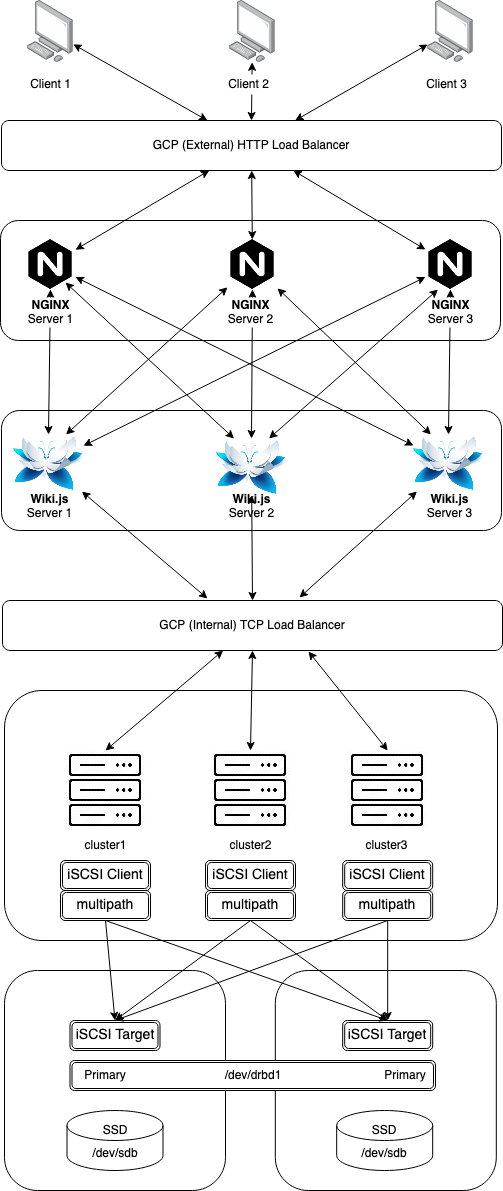
\includegraphics[width=0.54\linewidth]{img/wiki_deploy.png}
    \caption{Arquitetura Implementada}
    \label{fig:final-arch}
\end{figure}


\subsection{Testes de Carga}

Uma vez implementada a topologia apresentada na Figura \ref{fig:final-arch}, voltámos a realizar os mesmos teste de carga já referidos, mas desta vez nesta nova arquitectura de alta disponibilidade e desempenho.

\textbf{Nota:} de referir que para facilitar a leitura e suprimir a necessidade de voltar atrás para se perceber qual o objetivo dos demais testes, as descrições apresentadas acima voltam a ser apresentadas nesta secção.

\subsubsection{Teste 1}

% Inicio do Teste 1 - Diogo Monteiro - BullDogChinês

Tal como previamente descrito, o teste 1 visa representar o cenário mais básico: um utilizador aceder à página inicial da wiki. Para a realização deste teste, irão ser utilizadas mais \textit{threads} do que nos restantes, dado que num cenário real, o acesso à página inicial da wiki será a ação mais comum. O método que será testado é o seguinte:

\begin{enumerate}
  \item GET /
\end{enumerate}

O teste foi corrido com 100, 1000, 5000 e 10000 \textit{threads} (utilizadores), sendo que recorremos aos relatórios gerados pelo \textit{JMeter} para apresentar os seguintes resultados:

\begin{table}[h!]
\centering
    \begin{tabular}{ |c|c|c|c|  }
        \hline
        \multicolumn{4}{|c|}{Página Inicial} \\
        \hline
         Threads & Erro & Tempo Resposta Médio (ms) & \textit{Throughput (Trans./s)}\\
        \hline
        100   & 0.00\%   & 	89.32  & 98.81 \\
        1000  & 0.00\%   & 2929.41 & 124.64	\\
        5000  & 35.20\%  & 14183.61 & 132.07 \\
        10000 & 53.29\%  & 18069.55 & 199.77 \\
        \hline
    \end{tabular}
    \caption{Deployment - Sumário do Teste 1}
    \label{table:1}
\end{table}

Realizando uma análise aos dados da tabela, podemos, novamente, verificar que nas situações em que utilizamos 100 e 1000 utilizadores não obtemos nenhuma percentagem de erro. À medida que esses valores sobem para a casa dos 5000 já começámos a obter uma percentagem significativa de erros, sendo que com 10000 essa percentagem é ainda maior. Esta situação também se repetia na tipologia anterior, porém, em comparação, a percentagem de erros desta versão sofreu uma redução considerável em ambos os casos.

Para além disso e tal como esperado, o aumento do número de threads provocou tanto o aumento do \textit{throughput} como dos tempos médios de resposta da aplicação. Tal como no caso da percentagem de erros, comparativamente à versão anterior, ambos os valores sofreram uma \textbf{enorme} melhoria.\\
\\

\begin{figure}[ht!]
    \centering
    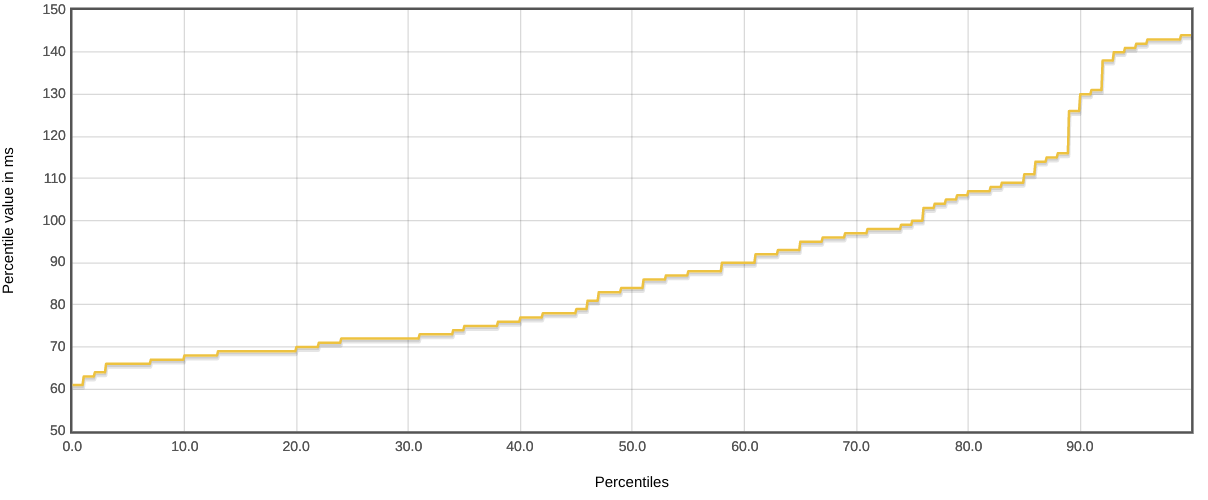
\includegraphics[width=.45\linewidth]{img/testes/i2-t1-100.png}
    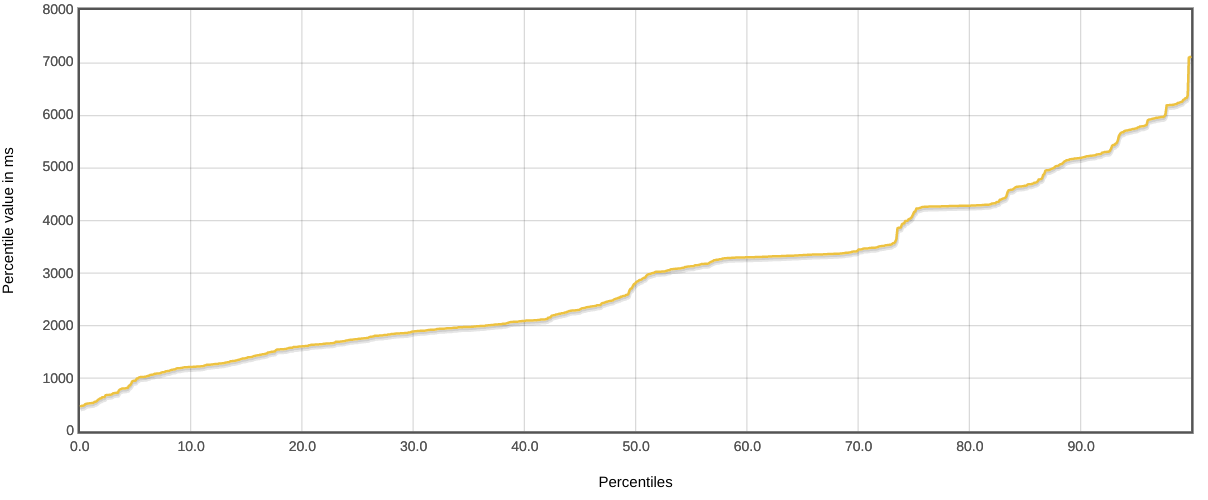
\includegraphics[width=.45\linewidth]{img/testes/i2-t1-1000.png}
    \caption{Percentil Tempo de Resposta para 100 e 1000 Threads}
\end{figure}

\begin{figure}[ht!]
    \centering
    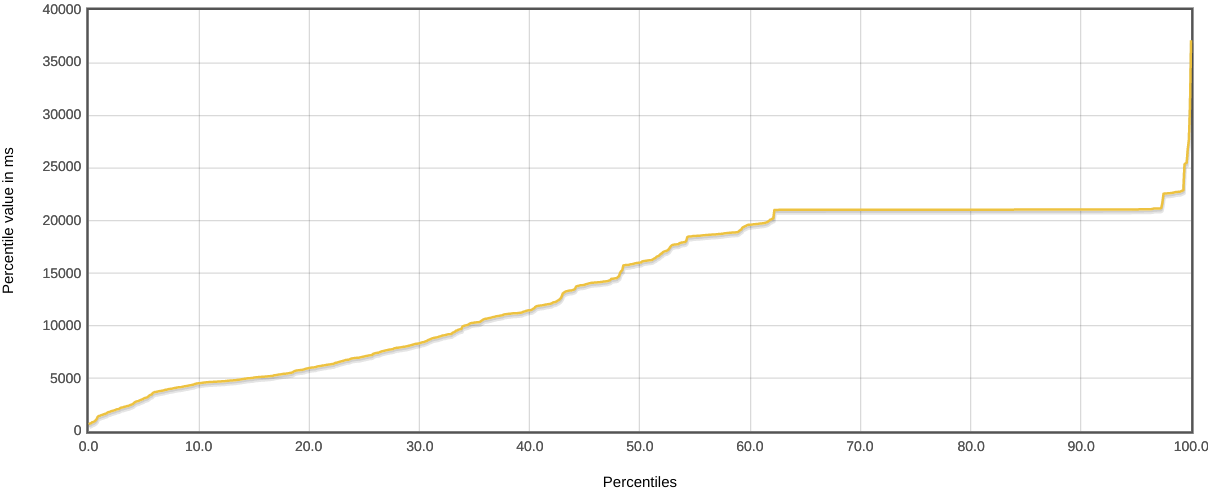
\includegraphics[width=.45\linewidth]{img/testes/i2-t1-5000.png}
    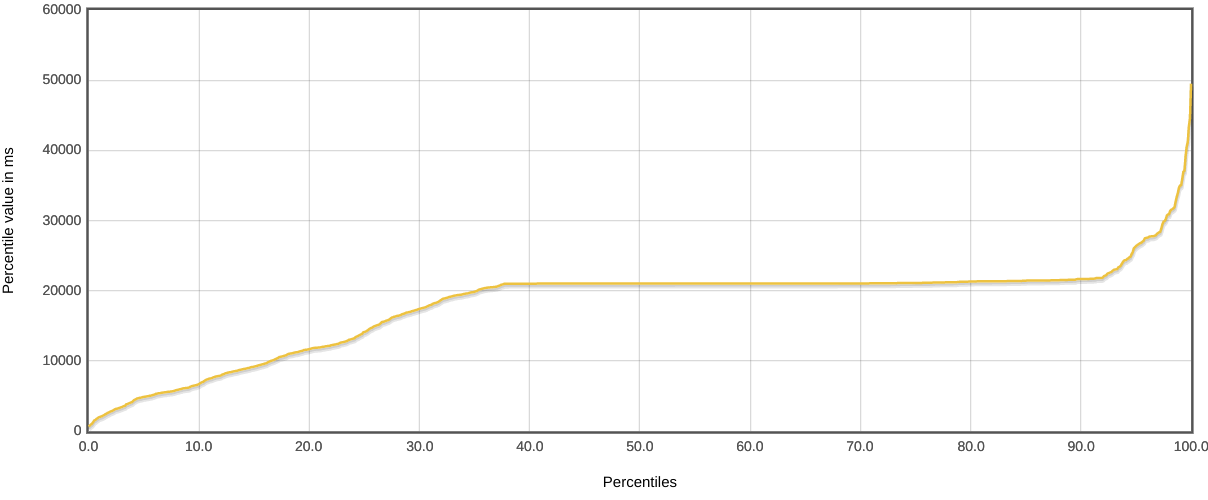
\includegraphics[width=.45\linewidth]{img/testes/i2-t1-10000.png}
    \caption{Percentil Tempo de Resposta para 5000 e 10000 Threads}
\end{figure}

Por fim, este primeiro teste veio demonstrar que contrariamente à implementação anterior, a nova arquitectura, que implementámos, é capaz de fornecer tempos de resposta perfeitamente aceitáveis, mas com uma percentagem de erro que, apesar de ter sofrido uma melhoria considerável, permanece alta.

% Fim do Teste 1 - Diogo Monteiro - BullDogChinês

\subsubsection{Teste 2}

O Teste 2 visa representar o cenário em que um utilizador entra na página inicial, navegando de seguida para uma outra página da wiki. Neste caso em específico, todas as \textit{threads} abrem a mesma página após pedirem a página inicial e esperarem 1000 milissegundos. Ao correr este teste são testados os seguintes métodos:

\begin{enumerate}
  \item GET /
  \item GET /en/ICD
\end{enumerate}

O teste foi corrido com 1000 e 5000 \textit{threads}, sendo que recorremos aos relatórios gerados pelo \textit{JMeter} para apresentar os seguintes resultados. Estes valores foram escolhidos pela sua relevância tendo em conta o teste anterior.

\begin{table}[h!]
\centering
    \begin{tabular}{ |c|c|c|c|c|  }
        \hline
        \multicolumn{4}{|c|}{Página Inicial} \\
        \hline
         Threads & Erro & Tempo Resposta Médio (ms) & \textit{Throughput (Trans./s)}\\
        \hline
        1000  & 0.00\%   & 1439.57  & 201.03\\
        5000  & 24.26\%  & 9570.59 & 226.88\\
        \hline
    \end{tabular}
    \caption{Deployment - Sumário do Teste 2}
    \label{table:1}
\end{table}

Analisando os dados da tabela, podemos verificar que com 1000 utilizadores não obtemos nenhuma percentagem de erro. Quando aumentamos para valores na casa dos 5000 começámos a obter uma percentagem significativa de erros.

Ao aumentar o número de threads, verificámos também o aumento do \textit{Throughput} da aplicação, bem como do tempo de resposta médio aos pedidos. Este último valor, dado que também serve de medida de performance do sistema, mostra-nos que nos casos em que assegurámos que todos os pedidos são atendidos, estes esperam uma quantidade de tempo considerável. 

Em relação à arquitectura inicial, podemos ver que o tempo de resposta médio diminui drasticamente para ambos os números de threads, bem como o aumento do \textit{throughput}. No entanto, este último teve valores semelhantes para número de threads diferentes, o que não acontecia anteriormente. A percentagem de erros também diminui significativamente, para metade no caso das 5000 threads. 

\begin{figure}[ht!]
    \centering
    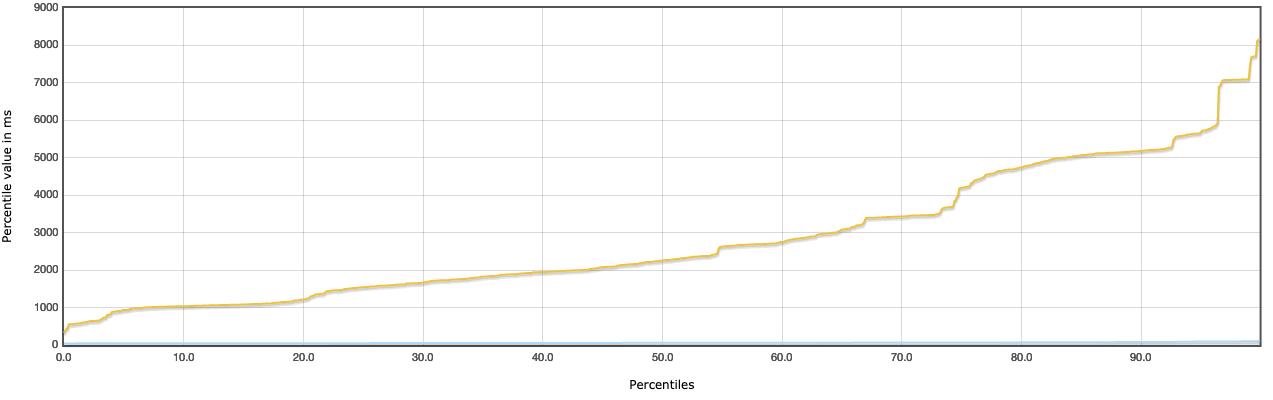
\includegraphics[width=.45\linewidth]{img/testes/i2-t2-1000.png}
    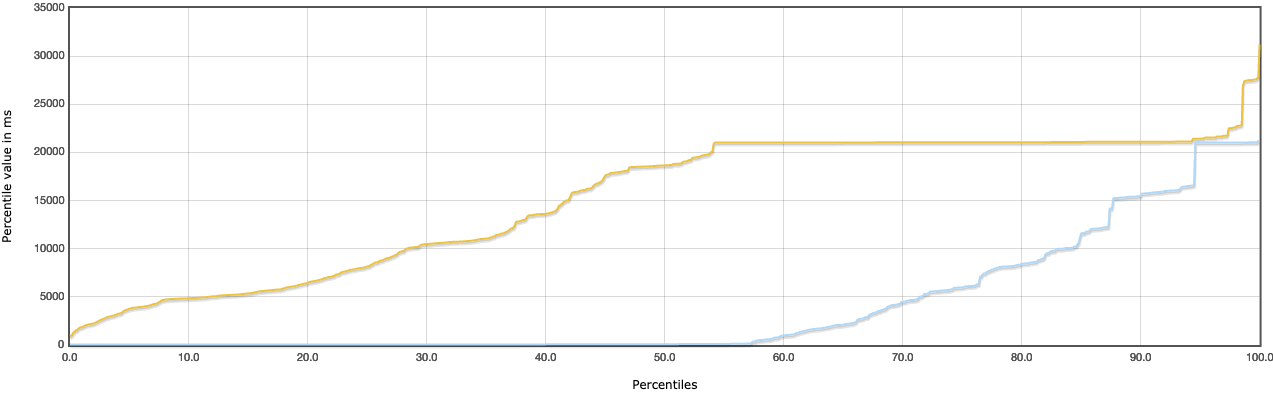
\includegraphics[width=.45\linewidth]{img/testes/i2-t2-5000.png}
    \caption{Percentil Tempo de Resposta para 1000 e 5000 Threads}
\end{figure}

Verificando os gráficos apresentados, em que a linha azul representa os pedidos referentes à página de teste e a linha laranja os pedidos referentes à página inicial. Ao contrário da arquitectura inicial, podemos ver que há agora uma grande diferença de tempos de resposta entre as duas operações.

\subsubsection{Teste 3}

O Teste 3 visa representar o cenário em que um administrador efetua login no sistema, sendo redirecionado para a página principal. Ao correr este teste são testados os seguintes métodos:

\begin{enumerate}
  \item GET  /login
  \item POST /graphql
  \item GET  /
\end{enumerate}

O teste foi corrido com 100, 250, 500, 1000 e 5000 \textit{threads}, sendo que recorremos aos relatórios gerados pelo JMeter para apresentar os seguintes resultados.
O processo de login é constituido pelos 3 pedidos apresentados, sendo que o conteúdo do POST que é feito possui o endereço de email e a password da conta utilizada no teste. Estes 3 pedidos foram encapsulados num processo mais generalizado que representa o login como um todo. Optámos por esta visão de modo a representar de modo mais fidedigno o ato de efetuar login, dado que não é possível efetuar login se uma das operações falhar. Outra atenção que tivemos, foi o cancelamento de uma \textit{thread} no caso de um dos pedidos falhar.

\begin{table}[h!]
\centering
    \begin{tabular}{ |c|c|c|c|c|  }
        \hline
        \multicolumn{4}{|c|}{Página Inicial} \\
        \hline
         Threads & Erro & Tempo Resposta Médio (ms) & \textit{Throughput (Trans./s)}\\
        \hline
        100   & 0.00\%   & 1987.23  & 39.48\\
        250   & 0.00\%   & 2397.48  & 83.31\\
        500   & 0.00\%   & 2951.27 & 124.53\\
        1000  & 0.00\%   & 3185.77 & 120.18\\
        5000  & 25.78\%  & 12737.36 & 95.51\\
        \hline
    \end{tabular}
    \caption{Deployment - Sumário do Teste 3}
    \label{table:1}
\end{table}

Analisando os dados da tabela, podemos verificar que com 100, 250, 500 e 1000 não obtemos nenhuma percentagem de erro. Ao aumentar o número de threads, verificámos também o aumento do \textit{Throughput} da aplicação até um certo ponto, sendo que começou a diminuir a partir das 1000 threads. O tempo de resposta médio aos pedidos por sua vez não estagnou, subindo para valores elevados, mesmo sem a ocorrência de erros.

Em relação à arquitectura inicial, podemos ver que o tempo de resposta médio diminui drasticamente para todas as threads, bem como o aumento do \textit{throughput}, apesar deste começar a diminuir a certo ponto. Isto significa que a partir de um dado ponto a performance se começa a degradar acentuadamente. Quanto à percentagem de erros conseguimos eliminar por completo no caso das 1000 threads enquanto que na de 5000 obtemos resultados 2.5 vezes melhores. 

Nos gráficos apresentados, as \textbf{linhas vermelhas} representam o pedido \textbf{GET /login}, as \textbf{linhas azuis} representam o pedido \textbf{POST /graphql}, as \textbf{linhas amarelas} representam o pedido \textbf{GET /} e as \textbf{linhas verdes} representam o \textbf{Login} como um todo.


\begin{figure}[ht!]
    \centering
    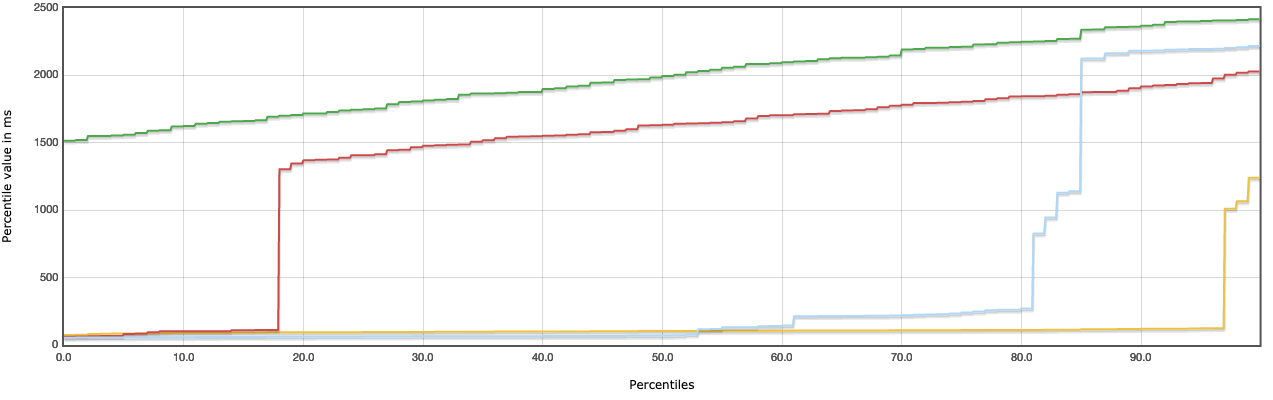
\includegraphics[width=.45\linewidth]{img/testes/i2-t3-100.png}
    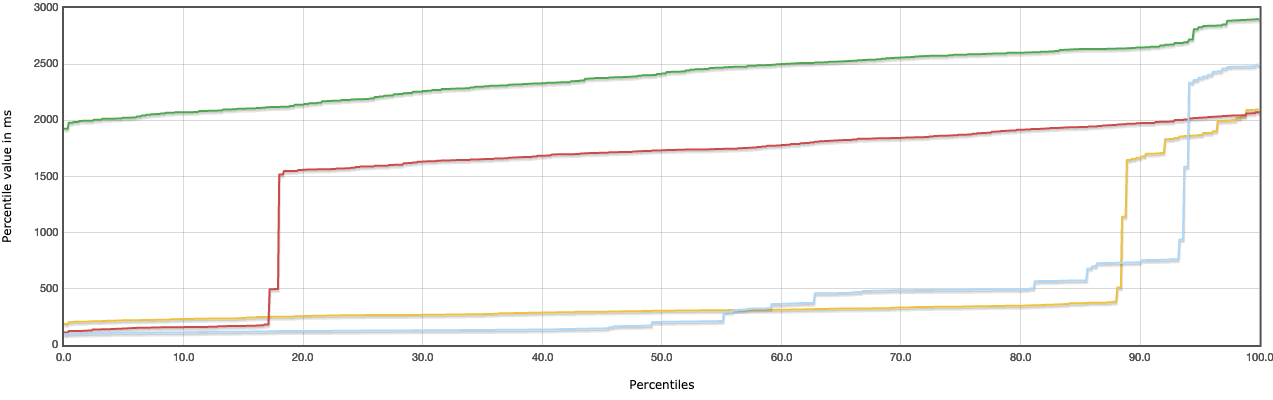
\includegraphics[width=.45\linewidth]{img/testes/i2-t3-250.png}
    \caption{Percentil Tempo de Resposta para 100 e 250 Threads}
\end{figure}

\begin{figure}[ht!]
    \centering
    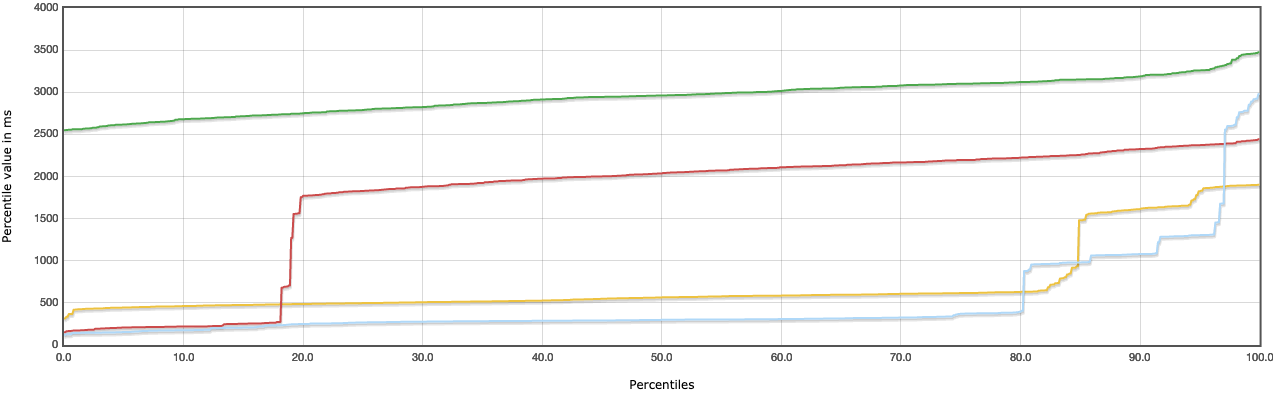
\includegraphics[width=.45\linewidth]{img/testes/i2-t3-500.png}
    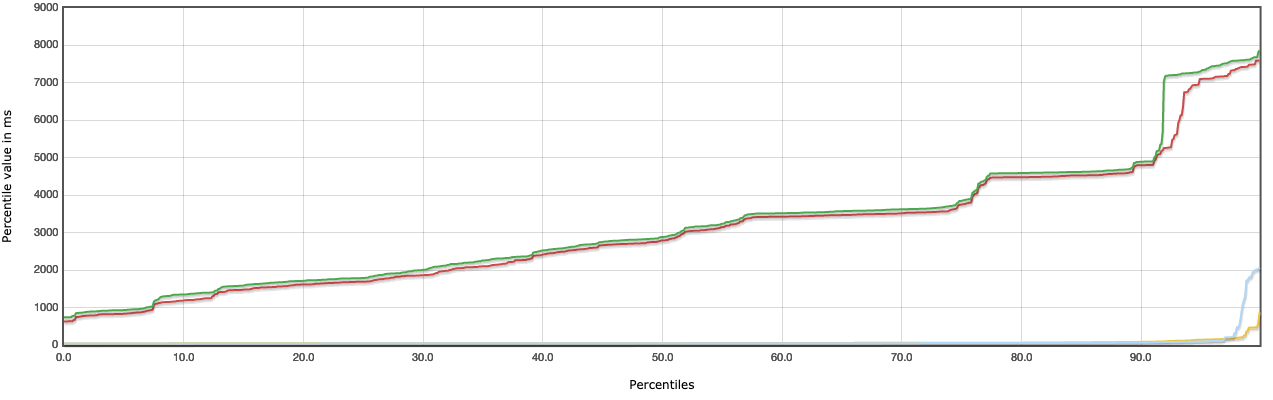
\includegraphics[width=.45\linewidth]{img/testes/i2-t3-1000.png}
    \caption{Percentil Tempo de Resposta para 500 e 1000 Threads}
\end{figure}

\begin{figure}[ht!]
    \centering
    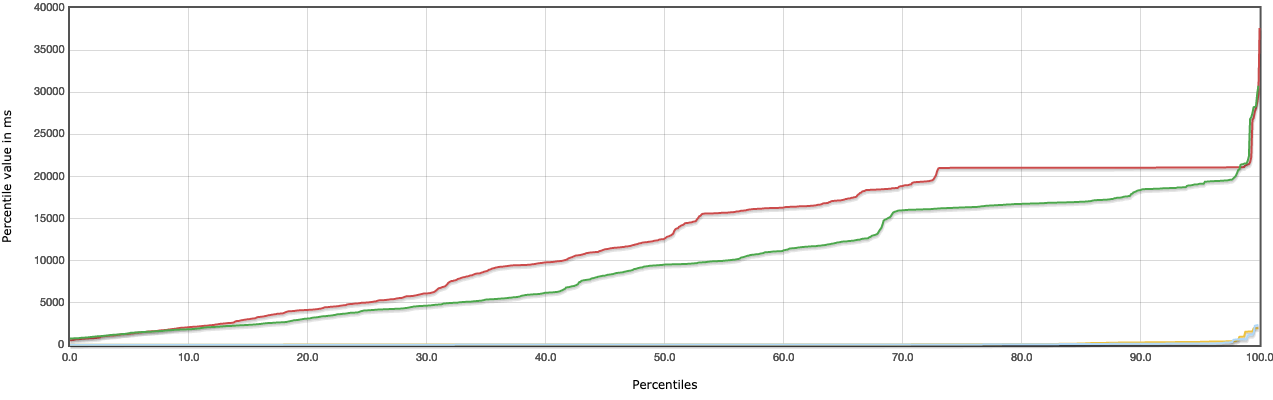
\includegraphics[width=.9\linewidth]{img/testes/i2-t3-5000.png}
    \caption{Percentil Tempo de Resposta para 5000 Threads}
\end{figure}

Ao contrário da arquitectura inicial, podemos ver que há agora uma grande diferença de tempos de resposta entre as operações. Anteriormente todas elas tinham a sua relevância enquanto que agora apenas as operações de LOGIN e GET LOGIN são comparativamente mais demoradas.

\subsubsection{Teste 4}

% Inicio do Teste 4 - Diogo Monteiro - BullDogChinês

O Teste 4 visa representar o cenário em que um administrador efetua login no sistema, sendo redireccionado para a página principal, seguido da criação de uma nova página wiki. Este teste irá testar os seguintes métodos:

\begin{enumerate}
    \item GET /login
    \item POST /graphql
    \item GET /
    \item GET /e/en/ThreadNum-Pagename
    \item POST /graphql
    \item GET /e/en/ThreadNum-Pagename
\end{enumerate}

Tal como explicado acima, nos métodos podemos encontrar as palavras \textit{ThreadNum} e \textit{Pagename}, que na verdade são variáveis. Cada \textit{thread} onde corremos os testes terá um \textit{ThreadNum} único, de maneira a conseguirmos saber que páginas cada \textit{thread} criou, e optamos por dar o nome à página a data do momento em que é criada em milissegundos para sabermos quando e por que ordem foram criadas as novas páginas. Isto é possível tomando partido das funções \texttt{\_\_time()} e \texttt{\_\_threadNum} do \textit{JMeter}.

O teste foi corrido com 100, 250 e 500 \textit{threads}, sendo que recorremos aos relatórios gerados pelo \textit{JMeter} para apresentar os seguintes resultados. A única diferença entre este teste e o anterior é que agora criamos uma página nova depois de fazermos o login, enquanto que no outro o teste acabaria precisamente depois de realizarmos o login. O processo de criação duma nova página é constituído pelos 3 últimos pedidos apresentados, sendo que o conteúdo do POST possui o conteúdo que a nova página irá apresentar. Estes 3 pedidos foram encapsulados num processo mais generalizado que representa a criação duma nova página como um todo. Optámos por esta visão de modo a representar de modo mais fidedigno o ato de criar uma nova página, dado que não é possível criá-la se uma das operações falhar. Sendo assim, preferimos separar a operação de efetuar login da criação da nova página para podermos avaliar individualmente cada um dos processos. 

\begin{table}[H]
\centering
\begin{tabular}{|c|c|c|p{3.5cm}|p{3cm}|}
\hline
Threads              & Operação & Erro    & Tempo Resposta Médio (ms) & \textit{Throughput (Trans./s)} \\ \hline
\multirow{2}{*}{100} & Login    & 0.00\%  & 3705.34                   & 37.645                          \\
                     & New Page & 0.00\% & 84141.29                 & 4,31                           \\ \hline
\multirow{2}{*}{250} & Login    & 0.00\%  & 3997.54                  & 46.75                          \\
                     & New Page & 0.00\% & 161938.23                 & 2.32                           \\ \hline
\multirow{2}{*}{500} & Login    & 0.00\%  & 6516.45                  & 17.14                         \\
                     & New Page & 0.00\% & 306854.25                 & 1.7                          \\ \hline
\end{tabular}
\caption{Deployment - Sumário do Teste 4}
\end{table}

Realizando uma análise aos dados recolhidos, podemos verificar que as operações de login continuam a ser realizadas sem qualquer erro. Porém, contrariamente à percentagem de erros que a versão anterior evidenciava, esta nova topologia reduz essa percentagem para 0 em todas as situações. Para além disto, esta nova versão apresenta uma estagnação quando o número de utilizadores cresce, começando a haver uma degradação nos tempos de resposta e começando o \textit{throughput} a cair. Isto leva-nos a crer que estamos a lidar com um número de utilizadores já acima da capacidade do sistema, começando os valores a ser pouco fidedignos.

Nos gráficos apresentados, as linhas \textbf{vermelho-escuro, roxo e amarelo-escuro} são as mais visíveis e ao mesmo tempo preocupantes, representando o \textbf{login, New Page e GET Page}, respetivamente.
\pagebreak

\begin{figure}[ht!]
    \centering
    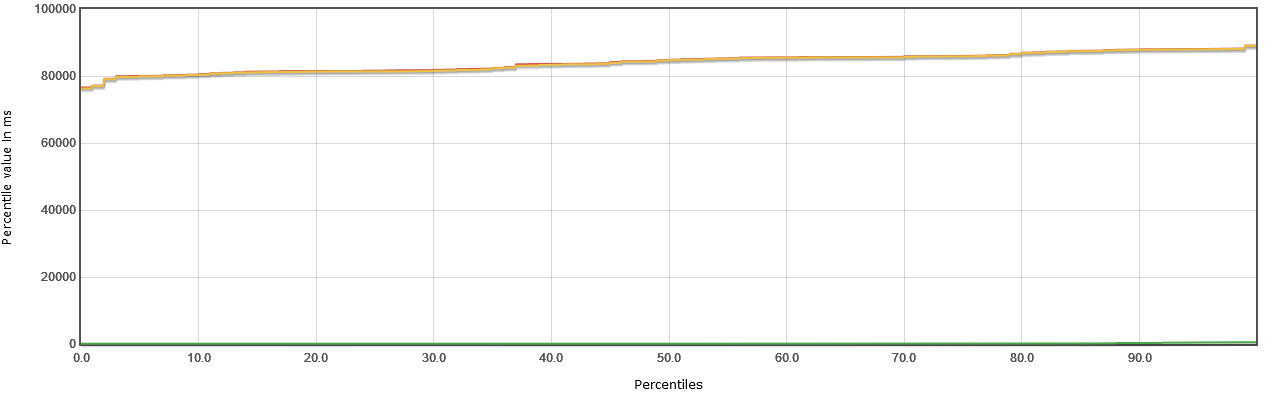
\includegraphics[width=.85\linewidth]{img/testes/i2-t4-100.png}
    \caption{Percentil Tempo de Resposta para 100 Threads}
\end{figure}

\begin{figure}[ht!]
    \centering
    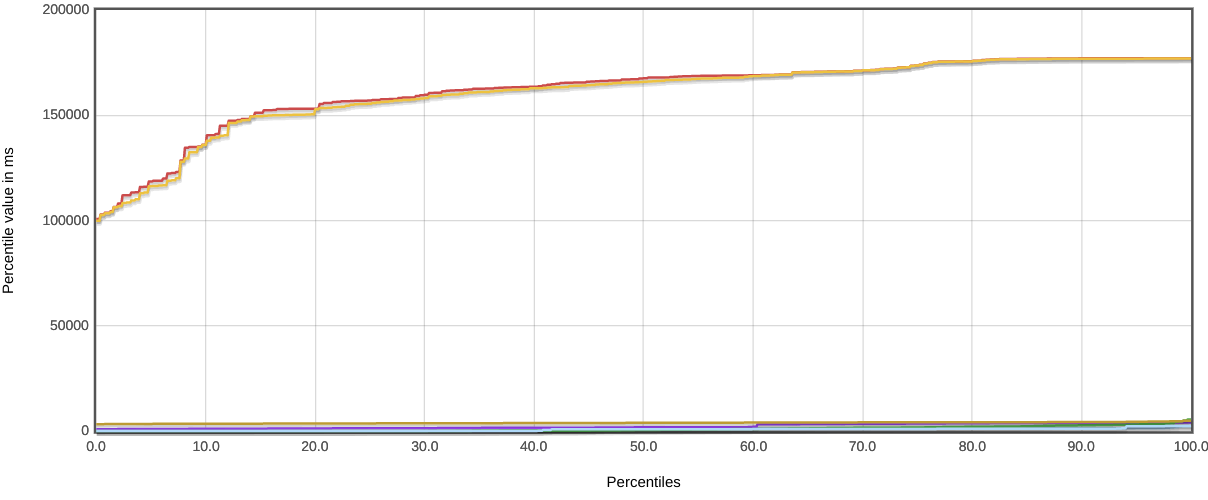
\includegraphics[width=.85\linewidth]{img/testes/i2-t4-250.png}
    \caption{Percentil Tempo de Resposta para 250 Threads}
\end{figure}

\begin{figure}[ht!]
    \centering
    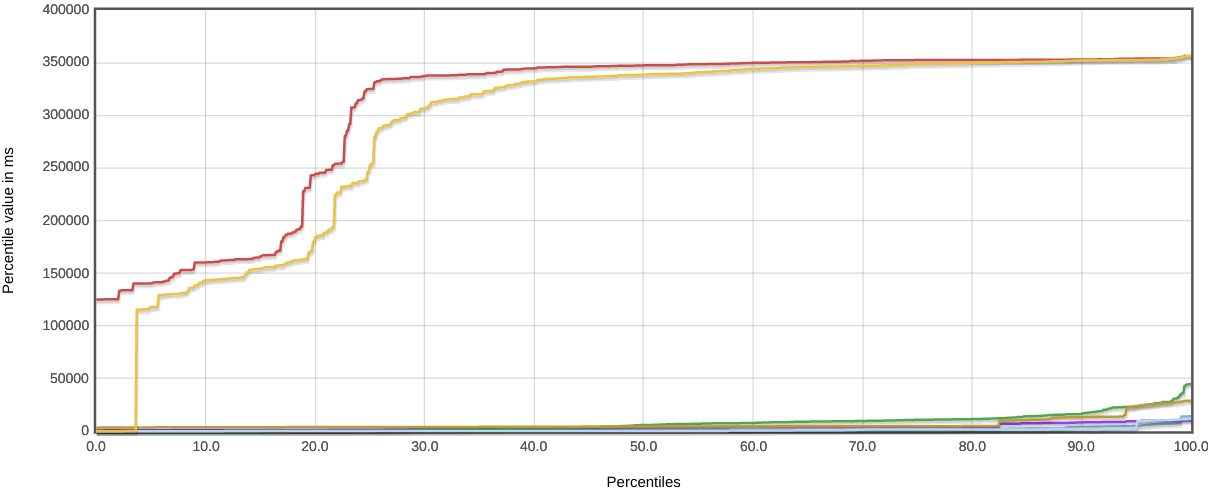
\includegraphics[width=.85\linewidth]{img/testes/i2-t4-500.png}
    \caption{Percentil Tempo de Resposta para 500 Threads}
\end{figure}

Em conclusão, no que diz respeito ao teste 4, esta nova topologia demonstra um excelente redução da percentagem de erro para a criação de uma nova página, mostrando assim uma melhoria na disponibilidade da plataforma. No entanto existem alguns aspetos a melhorar, nomeadamente a nível de performance, dado que gostaríamos de melhorar um pouco os tempos de resposta.

% VOLTAR A REVER O TESTE PARA AS 100 THREADS

% 100 THREADS ESTÁ MAL

% Fim do Teste 4 - Diogo Monteiro - BullDogChinês

\subsection{Análise de Desempenho}

% Não finalizado

Neste ponto, tendo uma arquitectura distribuída, é de esperar um aumento de disponibilidade e performance da aplicação, como foi mostrado anteriormente através da comparação dos resultados dos testes de carga das arquiteturas Inicial e Final. No entanto, apenas as camadas aplicacionais e web correm paralelamente, o que explica que as melhorias mais significativas sejam em pedidos menos dependentes da base de dados. Dado que o principal foco foi a disponibilidade do sistema, a principal alteração na camada de persistência foi a replicação do armazenamento. Isto apenas nos fornece redundância dos dados, não garantindo melhorias de performance em operações na base de dados. 

Olhando para o nosso principal objetivo, garantir elevada disponibilidade, podemos dizer que obtivemos sucesso, dado que todas as operações com uma percentagem de erro não nula diminuíram consideravelmente, e dado que o sistema é capaz de resistir a falhas de componentes. A nível de performance, os nossos testes de carga revelam que também obtivemos melhorias significativas, especialmente devido ao balanceamento de carga por parte das camadas \textit{web} e aplicacional.

\subsection{Mitigação dos Pontos Críticos do Sistema}

Após a implementação da plataforma e execução de testes de carga, podemos avaliar os pontos críticos identificados na secção 3.1.

Um dos pontos críticos identificados foi a possibilidade de uma ou mais componentes do sistema falharem, causando uma interrupção do serviço. Esse problema foi mitigado, dado que os dados se encontram replicados e nenhuma componente do sistema possui uma só instância.

Foram também mencionados pontos críticos no sistema sob a forma de \textit{bottlenecks}, tendo estes tendo sido maioritariamente mitigados. A nível dos servidores aplicacionais e \textit{web}, com o uso de um balanceador de carga, eliminámos o \textit{bottleneck} por completo. No entanto, na nossa base de dados, apesar das melhorias de performance, esta continua em parte a ser um \textit{bottleneck} do sistema, dado que as operações mais lentas estão diretamente relacionadas com pedidos feitos à mesma. A conclusão a que chegámos é que para melhorar a performance do sistema como um todo, a implementação da base de dados terá de ser diferente. Como o nosso principal foco é a disponibilidade, optámos por manter a nossa arquitetura dado que satisfaz os nossos requisitos. 

Apesar de resolver uma boa parte dos problemas existentes, existem alguns quer irão sempre persistir, e que por muito improváveis que possam ou não ser, devem ser considerados. Apesar de termos todas as componentes replicadas, se falharem os 3 nós do cluster de armazenamento em simultâneo, o nosso sistema irá falhar. O mesmo se aplica aos servidores NGINX e aos servidores Wiki.js, bem como às duas instâncias que compõem o drbd. Outro problema que poderá existir é o caso de um dos \textit{load balancers} falhar, tornando o nosso sistema inoperacional.

Resumindo, no caso de todas as instâncias de uma das camadas falharem ou de um dos \textit{load balancers} falhar, o nosso sistema ficará indisponível, apesar de se tratarem de situações improváveis. 

Visto isto, podemos afirmar que a arquitetura implementada garante elevada disponibilidade.

\pagebreak